
\section{Auswertung}
\subsection{Strömungsgeschwindigkeit}
Zu Beginn des Versuchs werden der Dopplerwinkel $\su{\alpha}$ für die drei Prismenwinkel
15$^\circ$, 30$^\circ$ und 60$^\circ$ mit Formel
\begin{equation*}
  \alpha = 90°-\arcsin\left(\sin\theta\cdot\frac{c_L}{c_P}\right)
\end{equation*}
berechnet.
$c_L$ ist die Schallgeschwindigkeit der Dopplerflüssigkeit und $c_P$ die des Prismamaterials.
Die berechneten Winkel sind in Tabelle \ref{tab:doppel} zu sehen.
\begin{table}
\centering
\caption{Doppelwinkel}
\label{tab:doppel}
\begin{tabular}{S S}
\toprule
{Prismenwinkel\,$\su{\theta}$} & {Dopplerwinkel\,$\su{\alpha}$} \\
\midrule
{$15^\circ$} & {$80,06^\circ$}  \\
{$30^\circ$} & {$70,53^\circ$}  \\
{$60^\circ$} & {$54,74^\circ$}  \\
\bottomrule
\end{tabular}
\end{table}
\newline
Durch das Umformen von Formel \ref{eqn:2} können die Strömungsgeschwindigkeiten der drei Rohre berechnet werden
\begin{equation}
    v_{\text{ström}} = \frac{\symup{\Delta} \nu \cdot c}{2 \, \nu_0 \, \symup{cos} \, \alpha} \, .
\end{equation}
Dabei ist $c = \SI{1800}{\meter\per\second}$ und $\nu_0 = \SI{2}{\mega\hertz}$ die verwendete Ultraschallsonde.
Die Ergebnisse für die Strömungsgeschwindigkeiten der einzelnen Rohre sind aus den Tabellen
\ref{tab:10mm}, \ref{tab:16mm} und \ref{tab:7mm} zu entnehmen.
\newline
Zur Berechnung der Strömungsgeschwindigkeiten und der Frequenzverschiebung wird der Betrag der
gemessen Frequenzen genommen, da die Ultraschallsonde bei einigen Prismen gegen die Flussrichtung
ausgerichtet war.
\begin{table}
\centering
\caption{Messwerte für Rohr $1=10\,\mathrm{mm}$}
\label{tab:10mm}
\begin{tabular}{S S S S S S S}
\toprule
{v\,/\,$\su{\frac{l}{min}}$} & {$15^\circ\,/\,\su{Hz}$} & {$v_\text{ström,15$^\circ$}$\,/\,$\su{\frac{m}{s}}$} & {$30^\circ\,/\,\su{Hz}$}
& {$v_\text{ström,30$^\circ$}$\,/\,$\su{\frac{m}{s}}$} & {$60^\circ\,/\,\su{Hz}$} & {$v_\text{ström,60$^\circ$}$\,/\,$\su{\frac{m}{s}}$}\\
\midrule
2,95 & 73 & 0,19 & 110 & 0,15 & 269 & 0,21 \\
3,21 & 98 & 0,26 & 134 & 0,18 & 208 & 0,16 \\
3,52 & 110 & 0,29 & 159 & 0,21 & 330 & 0,26 \\
4,21 & 159 & 0,41 & 220 & 0,30 & 488 & 0,38 \\
5,01 & 195 & 0,51 & 342 & 0,46 & 720 & 0,56 \\
\bottomrule
\end{tabular}
\end{table}
\begin{table}
\centering
\caption{Messwerte für Rohr $2=16\,\mathrm{mm}$}
\label{tab:16mm}
\begin{tabular}{S S S S S S S}
\toprule
{v\,/\,$\su{\frac{l}{min}}$} & {$15^\circ\,/\,\su{Hz}$} & {$v_\text{ström,15$^\circ$}$\,/\,$\su{\frac{m}{s}}$} & {$30^\circ\,/\,\su{Hz}$}
& {$v_\text{ström,30$^\circ$}$\,/\,$\su{\frac{m}{s}}$} & {$60^\circ\,/\,\su{Hz}$} & {$v_\text{ström,60$^\circ$}$\,/\,$\su{\frac{m}{s}}$}\\
\midrule
2,95 & 61 & 0,16 & 85 & 0,12 & 122 & 0,10 \\
3,21 & 73 & 0,19 & 122 & 0,17 & 134 & 0,10 \\
3,52 & 73 & 0,19 & 110 & 0,16 & 159 & 0,12 \\
4,21 & 85 & 0,22 & 134 & 0,19 & 220 & 0,17 \\
5,01 & 122 & 0,32 & 183 & 0,26 & 330 & 0,26 \\
\bottomrule
\end{tabular}
\end{table}
\begin{table}
\centering
\caption{Messwerte für Rohr $3=7\,\mathrm{mm}$}
\label{tab:7mm}
\begin{tabular}{S S S S S S S}
\toprule
{v\,/\,$\su{\frac{l}{min}}$} & {$15^\circ\,/\,\su{Hz}$} & {$v_\text{ström,15$^\circ$}$\,/\,$\su{\frac{m}{s}}$} & {$30^\circ\,/\,\su{Hz}$}
& {$v_\text{ström,30$^\circ$}$\,/\,$\su{\frac{m}{s}}$} & {$60^\circ\,/\,\su{Hz}$} & {$v_\text{ström,60$^\circ$}$\,/\,$\su{\frac{m}{s}}$}\\
\midrule
2,95 & 159 & 0,41 & 269 & 0,36 & 403 & 0,31 \\
3,21 & 171 & 0,45 & 281 & 0,38 & 513 & 0,40 \\
3,52 & 195 & 0,51 & 415 & 0,56 & 610 & 0,48 \\
4,21 & 281 & 0,73 & 513 & 0,69 & 867 & 0,68 \\
5,01 & 403 & 1,05 & 757 & 1,02 & 1251 & 0,98 \\
\bottomrule
\end{tabular}
\end{table}
\newpage
Die Strömgeschwindkeiten werden für die unterschiedlichen Prismenwinkel gegen den Quotienten
$\su{\frac{\Delta \nu}{cos \alpha}}$ in Abbildungen \ref{fig:rohr1}, \ref{fig:rohr2} und
\ref{fig:rohr3} aufgetragen.
\begin{figure}
  \centering
  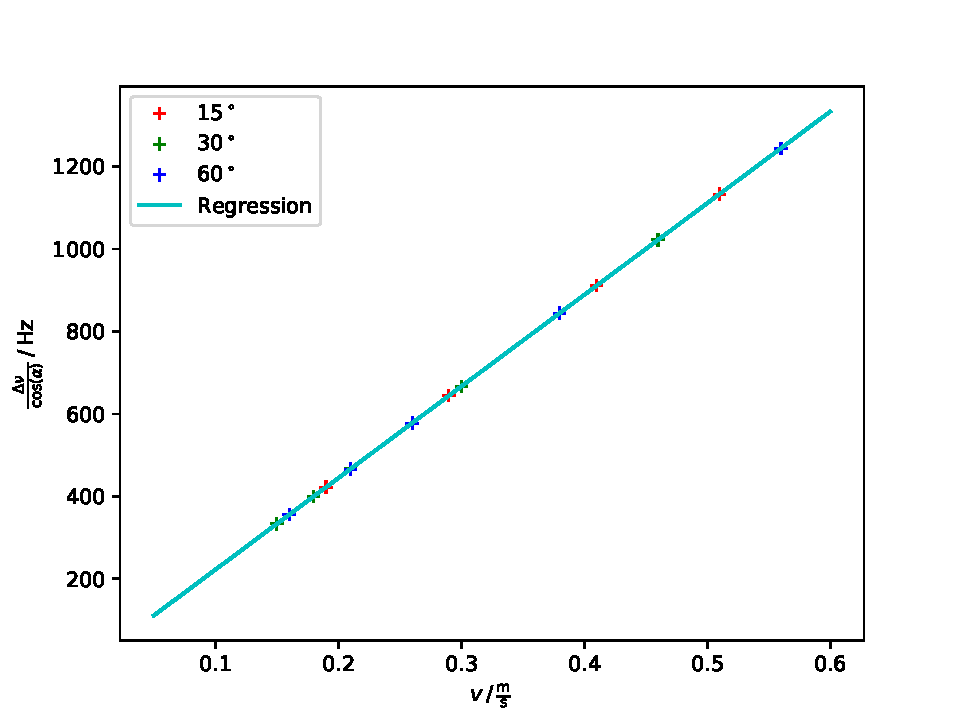
\includegraphics[scale=0.6]{rohr1.pdf}
  \caption{Rohr 1}
  \label{fig:rohr1}
\end{figure}
\begin{figure}
  \centering
  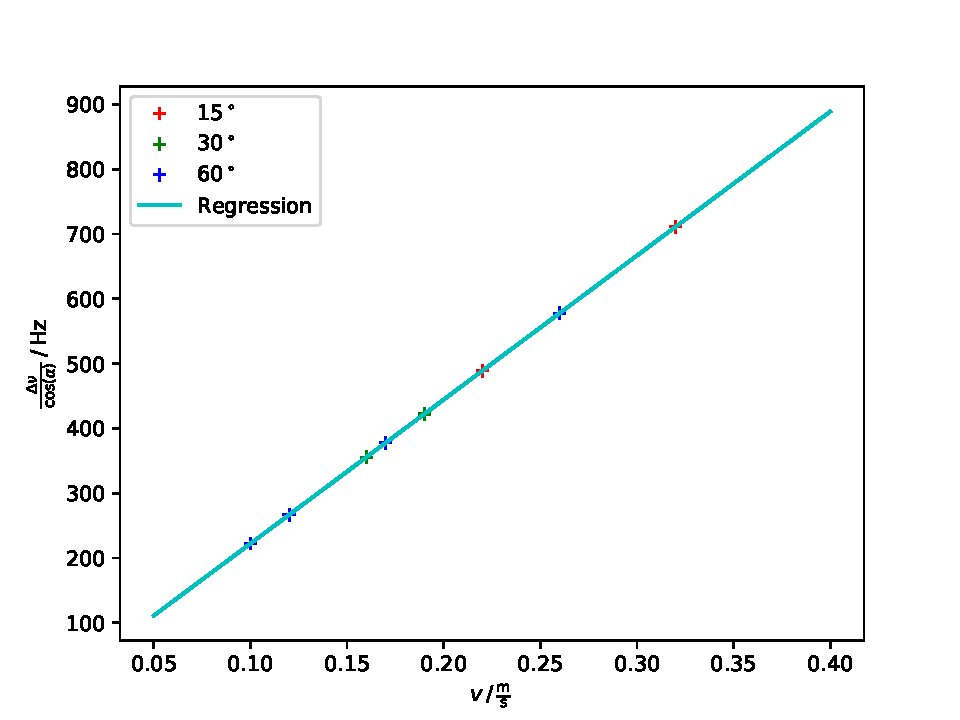
\includegraphics[scale=0.6]{rohr2.pdf}
  \caption{Rohr 2}
  \label{fig:rohr2}
\end{figure}
\begin{figure}
  \centering
  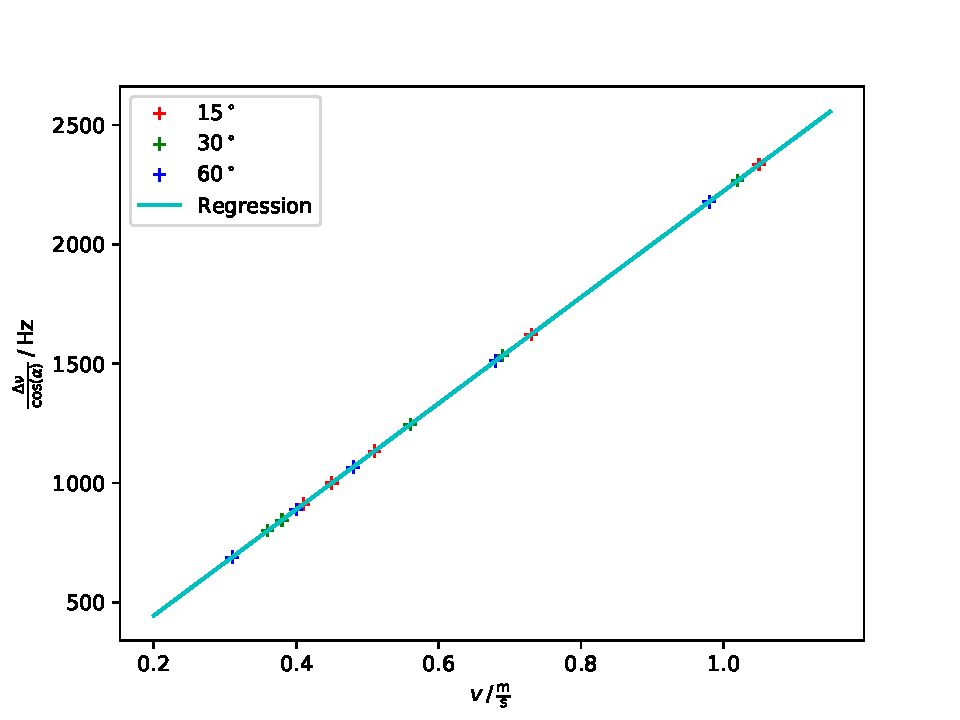
\includegraphics[scale=0.55]{rohr3.pdf}
  \caption{Rohr 3}
  \label{fig:rohr3}
\end{figure}
\newpage
\subsection{Strömungsprofil}
Durch den in der Anleitung angegeben Umrechnungsfaktor $4\symup{\mu s}= 10\,\mathrm{mm}$
ergibt sich, dass eine Messung erst ab einer Tiefe von $\symup{t}=30,7\,\mathrm{mm}=12,28\,\symup{\mu s}$
sinnvoll ist. Ab diesem Punkt tritt der Schall in die Dopplerflüssigkeit ein.
Deshalb wird im zweiten Versuchsteil die Messung bei einer Messtiefe von 12$\, \symup{\mu s}$ gestartet.
\newline
Die Messtiefe entspricht dem Beginn des Rohres mit $\su{s}=0\,\mathrm{mm}$. Die Messwerte
zur Bestimmung des Strömungsprofils bei einer Pumpleistung von 70\,\% sind in
Tabelle \ref{tab:70} angegeben, die für eine Pumpleistung von 45\,\% in Tabelle \ref{tab:45}.
\begin{table}[H]
  \small
  \caption{Messwerte bei einer Pumpleistung von 70\%}
  \label{tab:70}
  \centering
  \sisetup{table-format=1.1}
  \begin{tabular} {S S S S S}
    \midrule
    {Messtiefe $\:/\: \mu s$} & {Eindringtiefe\,/\,mm} &  {Strömunsgeschwindkeit} & {$\Delta \nu \:/\: \si{Hz}$} & {Streuintensität\,/\,$\%$} \\
    \midrule
    12,0 & 0,00 & 0,38 & 146 & 8,8 \\
    12,5 & 0,75 & 0,45 & 173 & 6,7 \\
    13,0 & 1,50 & 0,60 & 230 & 5,4 \\
    13,5 & 2,25 & 0,73 & 280 & 4,8 \\
    14,0 & 3,00 & 0,92 & 353 & 3,6 \\
    14,5 & 3,75 & 0,99 & 380 & 2,7 \\
    15,0 & 4,50 & 0,95 & 364 & 3,6 \\
    15,5 & 5,25 & 0,95 & 364 & 3,2 \\
    16,0 & 6,00 & 0,83 & 318 & 4,1 \\
    16,5 & 6,75 & 0,54 & 207 & 5,6 \\
    17,0 & 7,50 & 0,45 & 173 & 7,2 \\
    17,5 & 8,25 & 0,41 & 157 & 13,7 \\
    18,0 & 9,00 & 0,64 & 245 & 11,6 \\
    18,5 & 9,75 & 0,67 & 257 & 9,6 \\
    19,0 & 10,50 & 0,59 & 226 & 10,4 \\
  \end{tabular}
  \end{table}
  \begin{table}[H]
    \small
    \caption{Messdaten des Strömungsprofils 45.}
    \label{tab:45}
    \centering
    \sisetup{table-format=1.1}
    \begin{tabular} {S S S S S}
      \midrule
      {Messtiefe $\:/\: \mu s$} & {Eindringtiefe\,/\,mm} &  {$v_\text{ström}$\,/$\su{\frac{m}{s}}$} & {$\Delta \nu \:/\: \si{Hz}$} & {Streuintensität\,/\,$\%$} \\
      \midrule
      12,0 & 378 & 0,22 & 84 & 8,1 \\
      12,5 & 317 & 0,26 & 100 & 8,2 \\
      13,0 & 323 & 0,32 & 123 & 7,5 \\
      13,5 & 427 & 0,35 & 134 & 6,7 \\
      14,0 & 513 & 0,38 & 146 & 6,9 \\
      14,5 & 574 & 0,45 & 173 & 6,5 \\
      15,0 & 598 & 0,41 & 157 & 4,1 \\
      15,5 & 586 & 0,38 & 146 & 4,9 \\
      16,0 & 513 & 0,35 & 134 & 5,9 \\
      16,5 & 403 & 0,26 & 100 & 5,7 \\
      17,0 & 287 & 0,26 & 100 & 11,9 \\
      17,5 & 232 & 0,29 & 111 & 11,2 \\
      18,0 & 244 & 0,32 & 123 & 9,1 \\
      18,5 & 372 & 0,32 & 123 & 14,2 \\
      19,0 & 439 & 0,29 & 111 & 12,3\\
    \end{tabular}
    \end{table}
  \begin{figure}
      \centering
      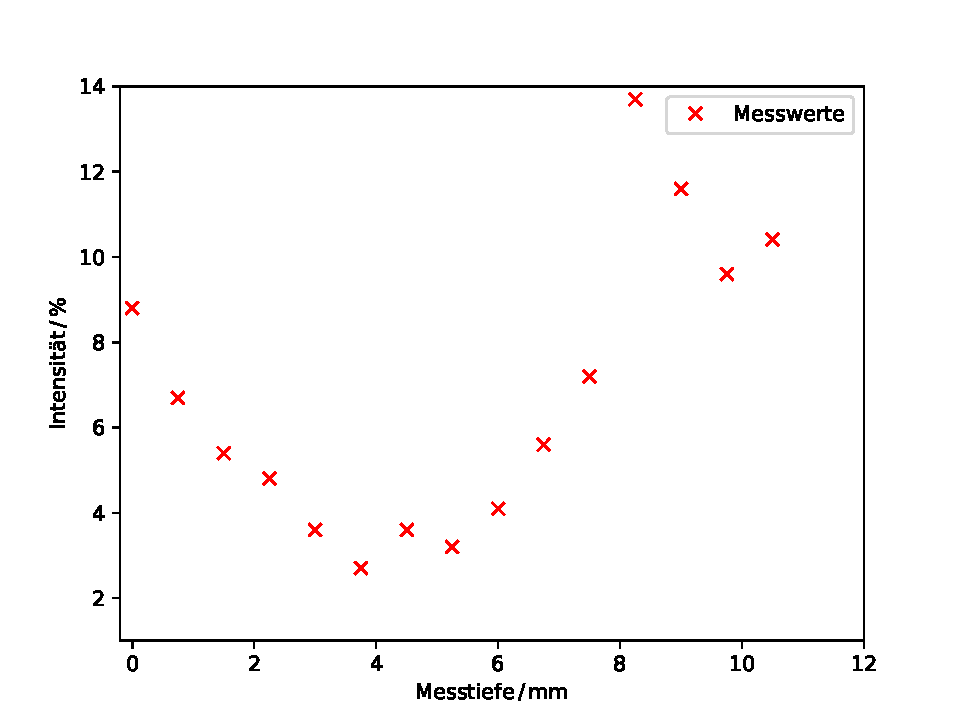
\includegraphics[scale=0.6]{pump70.pdf}
      \caption{Graphische Darstellung der Streuintensität in Abhängigkeit der Messtiefe bei einer Pumpleistung von 70\%.}
      \label{fig:pump70}
    \end{figure}
    \begin{figure}
        \centering
        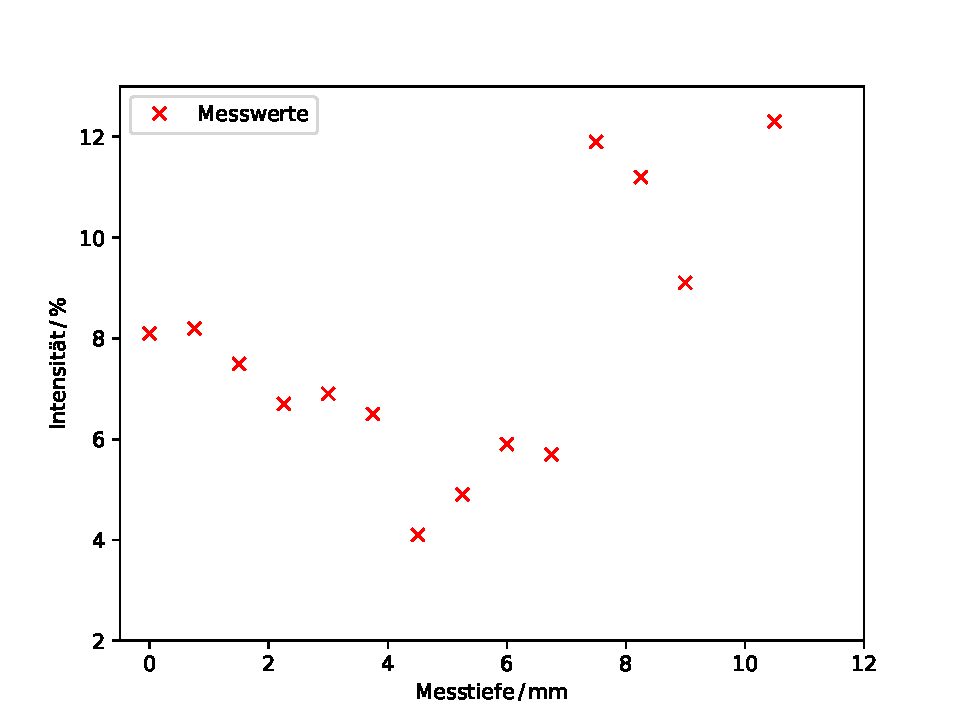
\includegraphics[scale=0.6]{pump45.pdf}
        \caption{Graphische Darstellung der Streuintensität in Abhängigkeit der Messtiefe bei einer Pumpleistung von 45\%.}
        \label{fig:pump45}
      \end{figure}
      \begin{figure}
          \centering
          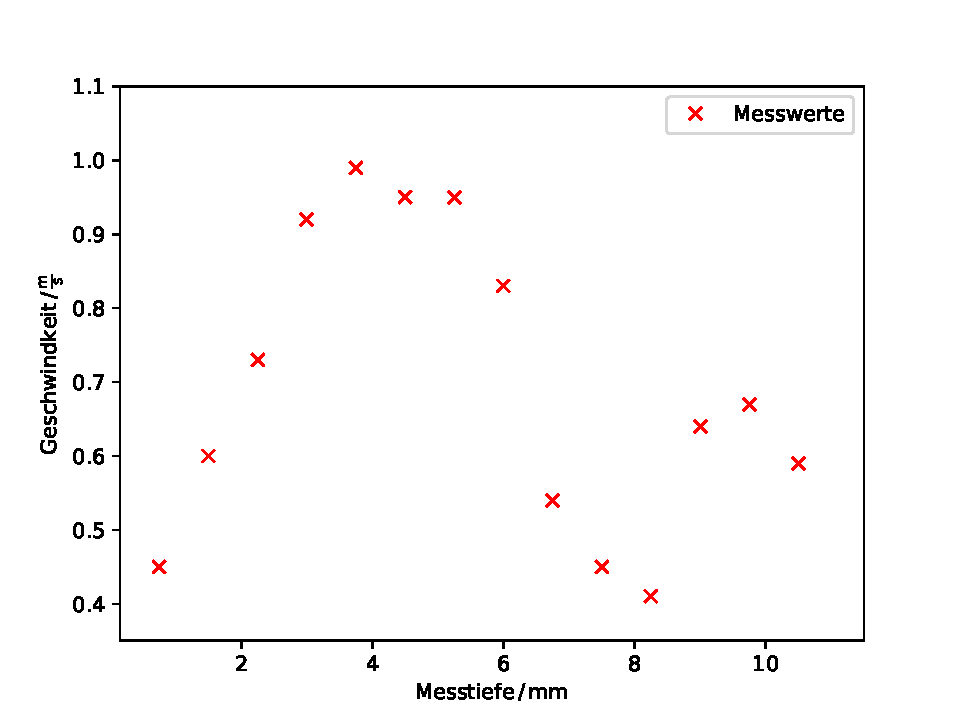
\includegraphics[scale=0.6]{pump70v.pdf}
          \caption{Graphische Darstellung der Geschwindigkeit in Abhängigkeit der Messtiefe bei einer Pumpleistung von 70\%.}
          \label{fig:pump70v}
        \end{figure}
        \begin{figure}
            \centering
            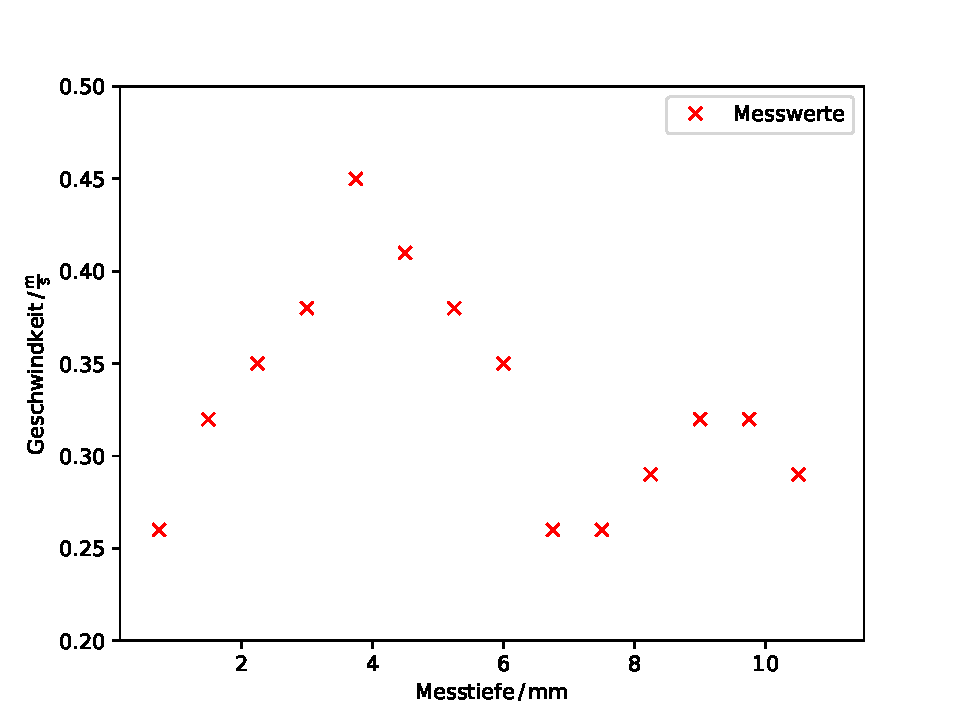
\includegraphics[scale=0.5]{pump45v.pdf}
            \caption{Graphische Darstellung der Geschwindigkeit in Abhängigkeit der Messtiefe bei einer Pumpleistung von 45\%.}
            \label{fig:pump45v}
          \end{figure}
\section{Diskussion}
Im ersten Versuchsteil ist deutlich die lineare Abhängigkeit der Strömungsgeschwindigkeit
vom Dopplerwinkel und der Frequenzverschiebung zu beobachten. Auch der Zusammenhang zwischen
Rohrradius und Strömgeschwindkeit wird mit diesem Experiment bestätigt. Mit zunehmenden Rohrradius
sinkt die Strömgeschwindkeit.

Im zweiten Versuchteil war das Ablesen der angezeigten Werte auf dem Computer
sehr schwierig, da sich die Werte innerhalb weinger Sekunden sehr stark veränderten.
Dadurch lassen sich die Abweichungen bei den Messungen der Frequenzverschiebung und
Streuintensität erklären. Daraus folgend kommt es auch zur Abweichung des parabolischen
Geschwindkeitprofils in dem Rohr. Der erneute Anstieg der Messwerte könnte auch aufgrund
des erneuten Schalleintritts in das Rohr erklärt werden.
